\documentclass[a4,openany,landscape,tikz]{article}
%\documentclass[11pt,a5,landscape,openany]{article}
\usepackage{xcolor}
\usepackage{makeidx}
\usepackage{geometry}       
\usepackage[chorded]{songs} 
\usepackage[colorlinks=true, pdfstartview=FitV, linkcolor=blue, citecolor=blue, urlcolor=blue]{hyperref} 
\usepackage{fancyhdr}
%\usepackage{abc}
%\usepackage{lilypond}
%\usepackage[parfill]{parskip}  
\usepackage{graphicx}
\usepackage{wrapfig}
\usepackage{qrcode}
%\usepackage{amssymb}
%\usepackage{epstopdf}
%\DeclareGraphicsRule{.tif}{png}{.png}{`convert #1 `dirname #1`/`basename #1 .tif`.png}

\usepackage{tikz}
\usetikzlibrary{decorations.text}


\setlength{\topmargin}{-0.5cm}
\setlength{\headheight}{0cm}
\setlength{\headsep}{-0.5cm}
\setlength{\textheight}{18cm}
\setlength{\textwidth}{24cm}
\setlength{\oddsidemargin}{-0.5cm}
\setlength{\evensidemargin}{-0.5cm}	
\setlength{\parindent}{0.25cm}
%\setlength{\parskip}{0.25cm}


\songpos{2}

%\pagestyle{fancy}
%\fancyhf{}
%\lfoot{%
%	\begin{minipage}{\textwidth}
%	\parbox{0.46\linewidth}{Some text to go in the footer Some text to go in the footer}\hfill
%	\parbox{0.70\linewidth}{\includegraphics[width=0.2\linewidth]{KK/KuylKamp_vierkantje_logo}}\hfill
%	\parbox{0.60\linewidth}{\raggedleft
\includegraphics[width=0.2\linewidth]{KK/KuylKamp_naam}}\hfill
%	\parbox{0.02\linewidth}{\raggedleft \thepage}%
%	\end{minipage}
%}

\renewcommand\printchord[1]{{\color{red!70!black}#1}}

\renewcommand{\songchapter}{\subsection}
\renewcommand{\songsection}{\subsection}

\newcommand{\U}{\Uparrow}
\newcommand{\D}{\Downarrow}


% ------------------- Title and Author -----------------------------
\title{AMeeSpeel KuylKampVuur Songbook 2016}

\author{gathered by Grobozeak-KKVO}
%\newindex{titleidx}{titleidx}
%\newauthorindex{authidx}{authidx}

%\frontmatter

\begin{document}
%\songcolumns{2}

\maketitle 

%\qrcode[hyperlink]{https://www.kuylkamp.nl}

%\parbox{0.70\linewidth}{\includegraphics[width=0.2\linewidth]{KK/KuylKamp_vierkantje_logo}}\hfill

 
\begin{wrapfigure}{l}{0.20\textwidth}
\qrcode[hyperlink]{https://github.com/coentjo/songbooks/releases}

%\url{https://github.com/coentjo/songbooks/releases}. 
\end{wrapfigure}


Bij een aantal nummers is aangegeven op welke positie de capo moet staan om met het origineel mee te kunnen spelen (als je het bijvoorbeeld op youtube opzoekt). Op het KuylKamp zullen we zoveel mogelijk \emph{zonder} spelen.  

Dit songbook is ook te vinden op internet, verstopt achter de URL \url{https://github.com/coentjo/songbooks/releases}. 

Op die internetpagina staan ook een aantal links naar opnamen van een aantal nummers zoals ze ook in de map staan.  
Natuurlijk heb je een gestemde gitaar nodig. Als je geen stemmer hebt kun je je mobiel gebruiken met een app: Zoek in de app store van je keuze op `\emph{Guitar Tuner}'. Zelf heb ik goeie ervaringen met `PitchLab Guitar Tuner' onder Android. 

Fouten, wijzigingen of andere tips? Geef ze door via email:   \href{mailto:coentjo@gmail.com}{coentjo@gmail.com} 

\begin{wrapfigure}{l}{0.25\textwidth}
\includegraphics[width=0.3\linewidth]{KK/KuylKamp_vierkantje_logo} 
\end{wrapfigure}


\begin{tikzpicture}[mypostaction/.style 2 args={
                         decoration={
                              text align={
                                    left indent=#1},
                                    text along path, 
                                    text={#2}
                                    },
                           decorate
                        }
                    ]
  \coordinate (specRoot) at (-10,0);
  \coordinate (testTreeRoot) at (0,0);
  \draw[-latex, blue!20!white, line width=5ex]  (specRoot) to[in=135,out=45] (testTreeRoot);

  \path [postaction={mypostaction={1cm}{Sla snel de bladzijde om}},
         postaction={mypostaction={1cm}{en begin met spelen!},
         /pgf/decoration/raise=-3mm}]
    (specRoot) to [in=120,out=45] (testTreeRoot);
\end{tikzpicture}

%\url{https://github.com/coentjo/songbooks/releases/download/v0.1/Amy_Green.Day.mp3}
%\qrcode{https://github.com/coentjo/songbooks/releases/download/v0.1/Amy_Green.Day.mp3}


%\tableofcontents 
%\showindex{Al hun liedjes}{titleidx}

%\showindex[2]{Nummers}{titleidx}
%\showindex[2]{artiesten}{authidx}


%\begin{abc}[name=c-dur]
%X: 1 % start of header
%K: C % scale: C major
%"Text"C4 G4 | (3FED c4 G2 |
%\end{abc}
%\newpage

\begin{songs}{} %{titleidx,authidx}

	\songcolumns{2}


	% Activate the following line by filling in the right side. If for example the name of the root file is Main.tex, write
% "...root = Main.tex" if the chapter file is in the same directory, and "...root = ../Main.tex" if the chapter is in a subdirectory.
 
%!TEX root = ../boktor.tex 

\beginsong{The wild rover}[by=Dubliners]
%\capo{3}
\begin{LARGE}
%\ \\
Ritme (3/4): $ \D . \ . \U \D \U $ \\
%\ \\
\end{LARGE}

%{\nolyrics Intro: \[E] \[G] \[A]}

\gtab{G}{320003}
\gtab{C}{332010}
\gtab{D7}{XX0232}



\beginverse
I've \[G]been a wild rover for many a \[C]year,   \brk   I \[G]spent all me \[C]money on \[D7]whiskey and \[G]beer
But \[G]now I'm returning with gold in great \[C]store,   \brk        And I \[G]never will \[C]play the wild \[D7]rover no \[G]more
\endverse



\beginchorus
  And it's \[D7]no nay never, \brk  \[klop klop klop] \[G]  \brk  no nay never no \[C]more
  Will I \[G]play the wild \[C]rover, no \[D7]never, no \[G]more
\endchorus



\beginverse
I \[G]went in to an alehouse I used to \[C]frequent,   \brk   And I \[G]told the land\[C]lady me \[D7]money was \[G]spent
I \[G]asked her for credit, she answered me \[C]`Nay!',   \brk   `Such \[G]custom as \[C]yours I could \[D7]have any \[G]day!'
\endverse



\beginchorus
  And it's \[D7]no nay never, \brk  \[klop klop klop] \[G]  \brk  no nay never no \[C]more
  Will I \[G]play the wild \[C]rover, no \[D7]never, no \[G]more
\endchorus



\beginverse
I \[G]took out of me pocket ten sovereigns \[C]bright,   \brk   And the \[G]landlady's \[C]eyes opened \[D7]wide with de\[G]light
She \[G]said: `I have whiskeys and wines on the \[C]best!,   \brk   And the \[G]words that I \[C]told you were \[D7]only in \[G]jest!'
\endverse



\beginchorus
  And it's \[D7]no nay never, \brk  \[klop klop klop] \[G]  \brk  no nay never no \[C]more
  Will I \[G]play the wild \[C]rover, no \[D7]never, no \[G]more
\endchorus



\beginverse
I'll go \[G]home to my parents, confess what I've \[C]done,   \brk   And \[G]ask them to \[C]pardon their \[D7]prodigal \[G]son
And \[G]when they've caressed me as oftimes be\[C]fore,   \brk   I \[G]never will \[C]play the wild \[D7]rover no \[G]more.
\endverse


\beginchorus
	(2x)
  And it's \[D7]no nay never, \brk  \[klop klop klop] \[G]  \brk  no nay never no \[C]more
  Will I \[G]play the wild \[C]rover, no \[D7]never, no \[G]more  
\endchorus



\endsong
					
	
		\beginscripture{(had een oud Chinees spreekwoord kunnen zijn)}
			Beter elke dag 5 minuten met in de hand een gitaar,
			
			Dan eenmaal per week een uur, 't is echt waar!
		\endscripture	
		
	
	% Activate the following line by filling in the right side. If for example the name of the root file is Main.tex, write
% "...root = Main.tex" if the chapter file is in the same directory, and "...root = ../Main.tex" if the chapter is in a subdirectory.
 

\beginsong{wonderwall (Kuylkamp: zonder capo) }[by=Oasis]
%\capo{3 voor originele hoogte, maar 

\begin{LARGE} 
Ritme: $ \D . \D . \D \U \D \U $  \\
\ \\
\end{LARGE} 


\gtab{Ex (Em7)}{022033}
\gtab{G}{320033}
\gtab{Dx (Dsus4)}{000233}
\brk
\gtab{Ax}{002033}
\gtab{Cx (Cadd9)}{X32033}
\gtab{F#x (G/F#)}{200233}


\beginverse
{\nolyrics Intro (2x): \[ Ex G Dx Ax ] }
\endverse


\beginverse
\[Ex] Today is \[G]gonna be the day,   \brk   That they're \[Dx]gonna throw it back to \[Ax]you
\[Ex] By now you \[G]should've somehow,   \brk   Rea\[Dx]lized what you gotta \[Ax]do
\[Ex]I don't believe that \[G]anybody,   \brk   \[Dx]Feels the way I \[Ax]do about you \[Ex]now \[G] \[Dx] \[Ax]
\endverse

\beginverse
\[Ex] Backbeat the \[G]word was on the street,   \brk   That the \[Dx]fire in your heart is \[Ax]out
\[Ex] I'm sure you've \[G]heard it all before,   \brk   But you \[Dx]never really had a \[Ax]doubt
\[Ex]I don't believe that \[G]anybody,   \brk   \[Dx]Feels the way I \[Ax]do about you \[Ex]now \[G] \[Dx] \[Ax]
\endverse

\beginchorus
And \[Cx]all the roads we \[Dx]have to walk are \[Ex]winding \[Ex], \brk  And \[Cx]all the lights that \[Dx]lead us there are \[Ex]blinding  \[Ex]
\[Cx]There are many \[Dx]things that I would \[G]like to \[F#x]say to \[Ex]you,   \brk But I don't know \[Dx]how  \[Ax]
\endchorus

\beginchorus
Because \[Cx]maybe  \[Ex] \[G],   \brk   You're \[Ex]gonna be the one that \[Cx]saves me \[Ex]  \[G]
And \[Ex]after all\[Cx]  \[Ex] \[G],   \brk   You're my \[Ex]wonderwall \[Cx]  \[Ex] \[G]
\endchorus

\beginverse
\[Ex] Today was \[G]gonna be the day,   \brk   But they'll \[Dx]never throw it back to \[Ax]you
\[Ex] By now you \[G]should've somehow,   \brk   Rea\[Dx]lized what you're not to \[Ax]do
\[Ex]I don't believe that \[G]anybody,   \brk   \[Dx]Feels the way I \[Ax]do about you \[Ex]now \[G] \[Dx] \[Ax]
\endverse

\beginchorus
And \[Cx]all the roads we \[Dx]have to walk are \[Ex]winding \[Ex], \brk  And \[Cx]all the lights that \[Dx]lead us there are \[Ex]blinding
\[Cx]There are many \[Dx]things that I would \[G]like to \[F#x]say to \[Ex]you,   \brk   But I don't know \[Dx]how  \[Ax]
\endchorus

\beginchorus
\rep{2}
I said \[Cx]maybe \[Ex] \[G] ,   \brk   You're \[Ex]gonna be the one that \[Cx]saves me \[Ex] \[G] 
And \[Ex]after \[Cx]all \[Ex] \[G] ,   \brk   You're my \[Ex]wonderwall  \[ Cx Ex G Ex ]
\endchorus

\beginchorus
I said \[Cx]maybe \[Ex] \[G] 
\rep{3}  You're \[Ex]gonna be the one that \[Cx]saves me \[Ex] \[G] 
\endchorus

\endsong
    \setcounter{songnum}{2}
	% Activate the following line by filling in the right side. If for example the name of the root file is Main.tex, write
% "...root = Main.tex" if the chapter file is in the same directory, and "...root = ../Main.tex" if the chapter is in a subdirectory.
 
%!TEX root = ../songbook.tex 

\beginsong{wonderwall }[by=Oasis]
\capo{3 voor originele hoogte, maar Kuylkamp: zonder capo} 

%\begin{LARGE} 
%Ritme: $ \D . \D . \D \U \D \U $  \\
%\ \\
%\end{LARGE} 


\gtab{Em7}{022033}
\gtab{G}{320033}
\gtab{Dsus4}{000233}
\brk
\gtab{Ax}{002033}
\gtab{Cadd9}{X32033}
\gtab{G/F#}{200233}


\beginverse
{\nolyrics Intro (2x): \[ Em7 G Dsus4 Ax ] }
\endverse


\beginverse
\[Em7] Today is \[G]gonna be the day,   \brk   That they're \[Dsus4]gonna throw it back to \[Ax]you
\[Em7] By now you \[G]should've somehow,   \brk   Rea\[Dsus4]lized what you gotta \[Ax]do
\[Em7]I don't believe that \[G]anybody,   \brk   \[Dsus4]Feels the way I \[Ax]do about you \[Em7]now \[G] \[Dsus4] \[Ax]
\endverse

\beginverse
\[Em7] Backbeat the \[G]word was on the street,   \brk   That the \[Dsus4]fire in your heart is \[Ax]out
\[Em7] I'm sure you've \[G]heard it all before,   \brk   But you \[Dsus4]never really had a \[Ax]doubt
\[Em7]I don't believe that \[G]anybody,   \brk   \[Dsus4]Feels the way I \[Ax]do about you \[Em7]now \[G] \[Dsus4] \[Ax]
\endverse

\beginchorus
And \[Cadd9]all the roads we \[Dsus4]have to walk are \[Em7]winding \[Em7], \brk  And \[Cadd9]all the lights that \[Dsus4]lead us there are \[Em7]blinding  \[Em7]
\[Cadd9]There are many \[Dsus4]things that I would \[G]like to \[G/F#]say to \[Em7]you,   \brk But I don't know \[Dsus4]how  \[Ax]
\endchorus

\beginchorus
Because \[Cadd9]maybe  \[Em7] \[G],   \brk   You're \[Em7]gonna be the one that \[Cadd9]saves me \[Em7]  \[G]
And \[Em7]after all\[Cadd9]  \[Em7] \[G],   \brk   You're my \[Em7]wonderwall \[Cadd9]  \[Em7] \[G]
\endchorus

\beginverse
\[Em7] Today was \[G]gonna be the day,   \brk   But they'll \[Dsus4]never throw it back to \[Ax]you
\[Em7] By now you \[G]should've somehow,   \brk   Rea\[Dsus4]lized what you're not to \[Ax]do
\[Em7]I don't believe that \[G]anybody,   \brk   \[Dsus4]Feels the way I \[Ax]do about you \[Em7]now \[G] \[Dsus4] \[Ax]
\endverse

\beginchorus
And \[Cadd9]all the roads we \[Dsus4]have to walk are \[Em7]winding \[Em7], \brk  And \[Cadd9]all the lights that \[Dsus4]lead us there are \[Em7]blinding
\[Cadd9]There are many \[Dsus4]things that I would \[G]like to \[G/F#]say to \[Em7]you,   \brk   But I don't know \[Dsus4]how  \[Ax]
\endchorus

\beginchorus
I said \[Cadd9]maybe \[Em7] \[G] ,   \brk   You're \[Em7]gonna be the one that \[Cadd9]saves me \[Em7] \[G] 
And \[Em7]after \[Cadd9]all \[Em7] \[G] ,   \brk   You're my \[Em7]wonderwall  \[ Cadd9 Em7 G Em7 ]
\endchorus

\beginchorus
I said \[Cadd9]maybe \[Em7] \[G] ,   \brk   You're \[Em7]gonna be the one that \[Cadd9]saves me \[Em7] \[G] 
And \[Em7]after \[Cadd9]all \[Em7] \[G] ,   \brk   You're my \[Em7]wonderwall  \[ Cadd9 Em7 G Em7 ]
\endchorus

\beginchorus
I said \[Cadd9]maybe \[Em7] \[G] 
\rep{3}  You're \[Em7]gonna be the one that \[Cadd9]saves me \[Em7] \[G] 
\endchorus

\endsong
 
	% Activate the following line by filling in the right side. If for example the name of the root file is Main.tex, write
% "...root = Main.tex" if the chapter file is in the same directory, and "...root = ../Main.tex" if the chapter is in a subdirectory.
 
%!TEX root = ../boktor.tex 

\beginsong{Brown eyed girl }[by=Van Morrison]


\begin{LARGE} 
Ritme: $ \D . \D \U . \ . \D . $  \\
\end{LARGE} 


\gtab{G}{320003}
\gtab{C}{332010}
\gtab{D}{XX0232}
\gtab{E}{022100}



\beginverse
\[G] Hey, where did we \[C]go
\[G] Days when the \[D]rain came
\[G] Down in the \[C]hollow
\[G] Playing a \[D]new game
\[G] Laughing, and a \[C]running, hey hey
\[G] Skipping and a \[D]jumping
\[G] In the misty \[C]morning fog with
\[G] Our \[D]hearts a thumpin' and \[C]you
\[D] My brown eyed \[G]girl  \[Em]
\[C] You\[D], my brown eyed \[G]girl \[D]
\endverse


\beginverse
\[G] Whatever \[C]happened 
to \[G] Tuesday and \[D]so slow
\[G] Going down the \[C]old mine with a 
\[G] transistor \[D]radio
\[G] Standing in the \[C]sunlight laughing
\[G] Hiding behind a \[D]rainbow's wall
\[G] Slipping and a \[C]sliding
\[G] All along the \[D]waterfall, with \[C]you
\[D] My brown eyed \[G]girl  \[Em]
\[C] You\[D], my brown eyed \[G]girl \[D]
\endverse

\beginchorus
\[D]Do you remember when we used to \[G]sing
Sha la la \[C]la la la la \[G]la la la la te \[D]da   Just like \[G]that
Sha la la \[C]la la la la \[G]la la la la te \[D]da   La te \[G]da
\endchorus


\beginverse
\[G] So hard to \[C]find my way
\[G] Now that I'm \[D]all on my own
\[G] I saw you just the \[C]other day
\[G] My, how \[D]you have grown
\[G] Cast my memory \[C]back there Lord
\[G] Sometimes I'm \[D]overcome thinkin' 'bout
\[G] Making love in the \[C]green grass, 
\[G] Behind the \[D]stadium, with \[C]you \[D]
My brown eyed \[G]girl \[Em]
\[C]You\[D], my brown eyed \[G]girl
\endverse

\beginchorus
\[D]Do you remember when we used to \[G]sing
(4x) Sha la la \[C]la la la la \[G]la la la la te \[D]da   Just like \[G]that
\endchorus



\endsong
 
	% Activate the following line by filling in the right side. If for example the name of the root file is Main.tex, write
% "...root = Main.tex" if the chapter file is in the same directory, and "...root = ../Main.tex" if the chapter is in a subdirectory.
 
%!TEX root = ../boktor.tex 

\beginsong{Country Roads}[by=John Denver]


%{\nolyrics Intro: \[E] \[G] \[A]}


\beginverse
Almost heaven, West Virginia
Blue ridge mountains, Shenandoah river
Life is old there, older than the trees
Younger than the mountains, growin' like a breeze
\endverse

\beginchorus
Country roads, take me home
To the place I belong
West Virginia, mountain momma
Take me home, country roads
\endchorus

\beginverse
All my memories, gather 'round her
Miner's lady, stranger to blue water
Dark and dusty, painted on the sky
Misty taste of moonshine, teardrops in my eyes
\endverse

\beginchorus
Country roads, take me home
To the place I belong
West Virginia, mountain momma
Take me home, country roads
\endchorus

\beginverse
I hear her voice in the mornin' hour she calls me
Radio reminds me of my home far away
Drivin' down the road I get a feelin'
That I should have been home yesterday, yesterday
\endverse

\beginchorus
\rep{2}
Country roads, take me home
To the place I belong
West Virginia, mountain momma
Take me home, country roads
\endchorus

\beginchorus
Take me home, country roads
Take me home, country roads
\endchorus


\endsong
					
	% Activate the following line by filling in the right side. If for example the name of the root file is Main.tex, write
% "...root = Main.tex" if the chapter file is in the same directory, and "...root = ../Main.tex" if the chapter is in a subdirectory.
 
%!TEX root = ../boktor.tex 

\beginsong{House of the rising sun}[]


\gtab{Am}{002210}
\gtab{C}{332010}
\gtab{D}{XX0232}

\gtab{F}{133211}
\gtab{E7}{020100}


\beginverse
There \[Am]is a \[C]house in \[D]New Or\[F]leans,
They \[Am]call the `\[C]Rising \[E7]Sun',
It's \[Am]been the \[C]ruin of \[D]many a poor \[F]boy
And \[Am]God, I \[E7]know, I'm \[Am]one \[C] \[D F Am E7 Am E7].
\endverse

\beginverse
My mother was a tailor,
She sewed my new blue jeans,
My father was a gambling man,
down in New Orleans.
\endverse

\beginverse
Now the only only thing a gambler needs
is a suitcase and a trunk 
and the only time he'll be satisfied
is when he's all a drunk
\endverse

\beginverse
Oh, mother, tell your children
Not to do what I have done -
Spend your lives in sin and misery
In the House of Rising Sun
\endverse

\beginverse
Well, I got one foot on the platform,
The other's on the train,
I'm going back to New Orleans,
to wear that ball and chain.
\endverse

\beginverse
%There \[Am]is a \[C]house in \[D]New Or\[F]leans,
%They \[Am]call the `\[C]Rising \[E7]Sun',
%It's \[Am]been the \[C]ruin of \[D]many a poor \[F]boy
%And \[Am]God, I \[E7]know, I'm \[Am]one \[C] \[D F Am E7 Am E7].
There is a house in New Orleans,
They call the `Rising Sun',
It's been the ruin of many a poor boy
And God, I know, I'm one.
\endverse



\endsong
 
	% Activate the following line by filling in the right side. If for example the name of the root file is Main.tex, write
% "...root = Main.tex" if the chapter file is in the same directory, and "...root = ../Main.tex" if the chapter is in a subdirectory.

%!TEX root = ../boktor.tex

\beginsong{Where did you sleep Last Night?}[by=nirvana]


%{\nolyrics Intro: \[E] \[G] \[A]}


\beginverse
My girl, my girl, don't lie to me, Tell me where did you sleep last night
In the pines, in the pines, Where the sun don't ever shine,
I would shiver the whole night through
\endverse

\beginverse
My girl, my girl, where will you go, I'm going where the cold wind blows
In the pines, in the pines, Where the sun don't ever shine,
I would shiver the whole night through
\endverse

\beginverse
Her husband, was a hard working man, Just about a mile from here
His head was found in a driving wheel, But his body never was found
My girl, my girl, don't lie to me
Tell me where did you sleep last night
In the pines, in the pines, Where the sun don't ever shine,
I would shiver the whole night through
\endverse

\beginverse
- Zwischenspiel -
\endverse

\beginverse
My girl, my girl, where will you go, I'm going where the cold wind blows
In the pines, in the pines, Where the sun don't ever shine
I would shiver the whole night through
\endverse

\beginverse
My girl, my girl, don't lie to me
Tell me where did you sleep last night
In the pines, in the pines, Where the sun don't ever shine
I would shiver the whole night through
\endverse

\beginverse
My girl, my girl, where will you go, I'm going where the cold wind blows
In the pines, the pines, The sun shines
I'll shiver ... the whole night through
\endverse

\endsong
 
	% Activate the following line by filling in the right side. If for example the name of the root file is Main.tex, write
% "...root = Main.tex" if the chapter file is in the same directory, and "...root = ../Main.tex" if the chapter is in a subdirectory.
 
%!TEX root = ../boktor.tex 

%\begin[quote,fragment,staffsize=26]{lilypond}


%\begin{lilypond}
%c d e f 
%\end{lilypond}


\beginsong{Come as you are }[by=Nirvana]


%{\nolyrics Intro: \[E] \[G] \[A]}

\beginverse
Come as you are, as you were
As I want you to be
As a friend, as a friend
As an old enemy

Take your time, hurry up
The choice is yours, don't be late
Take a rest as a friend
As an old
\endverse

\beginchorus
Memoria, memoria
Memoria, memoria
\endchorus

\beginverse
Come doused in mud, soaked in bleach
As I want you to be
As a trend, as a friend
As an old
\endverse

\beginchorus
Memoria, memoria
Memoria, memoria
\endchorus

\beginverse
And I swear that I don't have a gun
No I don't have a gun
No I don't have a gun
\endverse

\beginchorus
Memoria, memoria
Memoria, memoria
(No I don't have a gun)

And I swear that I don't have a gun
No I don't have a gun
No I don't have a gun
No I don't have a gun
No I don't have a gun

Memoria, memoria
\endchorus



\endsong
 
	% Activate the following line by filling in the right side. If for example the name of the root file is Main.tex, write
% "...root = Main.tex" if the chapter file is in the same directory, and "...root = ../Main.tex" if the chapter is in a subdirectory.
 
%!TEX root = ../boktor.tex 

\beginsong{Zombie }[by=Cranberries]

\gtab{Em}{022000}
\gtab{C}{332010}
\gtab{G}{320003}
\gtab{D}{XX0232}

%{\nolyrics Intro: \[E] \[G] \[A]}

\beginverse
intro (4x): \ \[ Em Cmaj7 G D ]
\endverse


\memorize
\beginverse
\[Em] Another h\[C]ead hangs lowly,   \brk   Ch\[G]ild is slowly \[D]taken
\[Em]And the violence \[C]caused such silence,   \brk   \[G]Who are we mis\[D]taken

But you \[Em]see it's not me,   \brk   It's not \[C]my family
In your \[G]head, in your head,   \brk   They are \[D]fighting
With their \[Em]tanks and their bombs,   \brk   And their \[C]bombs and their guns
In your \[G]head,   \brk   In your head they are \[D]cryin'
\endverse

\beginchorus
In your h\[Em]ead, in your \[C]head, , \brk  Zomb\[G]ie, zombie, zomb\[D]ie, Hey, hey
What's in your h\[Em]ead, in your h\[C]ead, , \brk  Zomb\[G]ie, zombie, zomb\[D]ie
\[Em] Hey, hey, hey, oh, \brk  \[C]Dou, dou, dou, dou
\[G]Dou, dou, dou, dou, \brk  \[D]Dou, dou, dou, dou
Dou, dou, dou, dou
\endchorus

\beginverse
^Another ^mother's breakin',   \brk   ^Heart is taking ^over
^When the violence ^causes silence,   \brk   ^We must be mis^taken

It's the ^same old theme since ^nineteen-sixteen
In your ^head,   \brk   In your head they're still ^fightin'
With their ^tanks and their bombs,   \brk   And their ^bombs and their guns
In your ^head, in your head they are ^dyin'
\endverse

\beginchorus
In your h\[Em]ead, in your \[C]head, , \brk  Zomb\[G]ie, zombie, zomb\[D]ie, Hey, hey
What's in your h\[Em]ead, in your h\[C]ead, , \brk  Zomb\[G]ie, zombie, zomb\[D]ie
\[Em]Hey, hey, hey, , \brk  \[C]Oh, oh, oh, 
\[G]oh, oh, oh, oh, \brk  Hey, oh, \[D]ya, ya-a 
\endchorus


\endsong
 
	% Activate the following line by filling in the right side. If for example the name of the root file is Main.tex, write
% "...root = Main.tex" if the chapter file is in the same directory, and "...root = ../Main.tex" if the chapter is in a subdirectory.
 
%!TEX root = ../boktor.tex 

\beginsong{The Needle and the Damage done }[by=Neil Young]

\gtab{D}{XX0232}
\gtab{Dx}{X30232}
\gtab{Dy}{X20030}
\gtab{Dz}{X10030}
\gtab{C}{332010}
\gtab{F}{X33210}
\gtab{E}{022100}


\beginverse
Intro: \rep{2}  {\nolyrics \[ D Dx Dy Dz C F E E ]}
\endverse

\memorize
\beginverse
\[D]I caught you knockin' at my \[Dx]cellar door
\[Dy]I love you, baby, can I \[Dz]have some more?
\[C]Ooh, \[F]ooh, the damage \[E]done \[E] 

\[D]I hit the city and I \[Dx]lost my band
\[Dy]I watched the needle take an\[Dz]other man
\[C]Gone, \[F]gone, the damage \[E]done \[E] 
\endverse

\beginverse
Instrumental: \rep{2}  {\nolyrics \[ D Dx Dy Dz C F E  ]}
\endverse

\beginverse
^I sing the song because I ^love the man
^I know that some of you don't ^understand
^Milk blood to keep from ^running out ^ 

^I've seen the needle and the ^damage done
^A little part of it in ^everyone
^But every junkie's like a ^settin' sun ^
\endverse

\beginverse
Instrumental: \rep{2}  {\nolyrics \[ D Dx Dy Dz C F E  ]}
\endverse


\endsong
 
	% Activate the following line by filling in the right side. If for example the name of the root file is Main.tex, write
% "...root = Main.tex" if the chapter file is in the same directory, and "...root = ../Main.tex" if the chapter is in a subdirectory.
 
%!TEX root = ../boktor.tex 

\beginsong{Happy Birthday }[by=traditional]


\gtab{G}{320003}
\gtab{D}{XX0232}
\gtab{C}{332010}

\textnote{op de plek van de puntjes naar believen de naam van een feestvierder roepen}

\beginverse
Happy \[G]Birthday to \[D]you
Happy \[D]Birthday to \[G]you
Happy \[G]Birthday 
Dear \[C]  ...
Happy \[G]Birthday \[D]to \[G]you
\endverse

\endsong
 
	% Activate the following line by filling in the right side. If for example the name of the root file is Main.tex, write
% "...root = Main.tex" if the chapter file is in the same directory, and "...root = ../Main.tex" if the chapter is in a subdirectory.
 
%!TEX root = ../boktor.tex 

\beginsong{Lang zal ze leven }[by=traditional]


%{\nolyrics Intro: \[E] \[G] \[A]}


\beginverse
\[G]Lang zal ze/hij leven
\[G]Lang zal ze/hij leven
\[G]Lang zal ze/hij leven in de \[D]gloria
In de \[G]glo\[C]ri\[G]a
\[C]In de \[G]glo\[D]ri\[G]a
\endverse

\endsong
 
	% Activate the following line by filling in the right side. If for example the name of the root file is Main.tex, write
% "...root = Main.tex" if the chapter file is in the same directory, and "...root = ../Main.tex" if the chapter is in a subdirectory.
 
%!TEX root = ../boktor.tex 

\beginsong{How you remind me }[by=Nickelback]
%capo{3}
%\gtab{X}{123456}
%\begin{LARGE}
%\ \\
%Ritme: $ \D . \D . \D . \D \U
%\ \\
% end{LARGE}

%{\nolyrics Intro: \[E] \[G] \[A]}


\beginverse
Never made it as a wise man
I couldn't cut it as a poor man stealing
Tired of living like a blind man
I'm sick of sight without a sense of feeling
And this is how you remind me
\endverse

\beginchorus
This is how you remind me
Of what I really am
This is how you remind me
Of what I really am

It's not like you to say sorry
(I) was waiting on a different story
This time I'm mistaken
For handing you a heart worth breaking

And I've been wrong, I've been down
Been to the bottom of every bottle
These five words in my head
Scream, "Are we having fun yet?"

(2x)  Yeah, yeah, yeah,  No, no
\endchorus

\beginverse
It's not like you didn't know that
I said I love you and I swear I still do
And it must have been so bad
Cause living with me must have damn near killed you
\endverse

\beginchorus
And this is how you remind me
. . .
. . .
%Of what I really am
%This is how you remind me
%Of what I really am

%It's not like you to say sorry
%I was waiting on a different story
%This time I'm mistaken
%For handing you a heart worth breaking

%And I've been wrong, I've been down
%Been to the bottom of every bottle
%These five words in my head
%Scream, "Are we having fun yet?"

\begin{Large}(4x) \end{Large}  Yeah, yeah, yeah,  No, no
\endchorus

\beginverse
Never made it as a wise man
I couldn't cut it as a poor man stealing
And this is how you remind me
This is how you remind me
\endverse

\beginchorus
This is how you remind me
. . . 
. . . 
%Of what I really am
%This is how you remind me
%Of what I really am

%It's not like you to say sorry
%I was waiting on a different story
%This time I'm mistaken
%For handing you a heart worth breaking

%And I've been wrong, I've been down
%Been to the bottom of every bottle
%These five words in my head
%Scream, "Are we having fun yet?"

(4x)  Yeah, yeah, yeah,  No, no
\endchorus

%\beginchorus
%\endchorus


\endsong
 
	% Activate the following line by filling in the right side. If for example the name of the root file is Main.tex, write
% "...root = Main.tex" if the chapter file is in the same directory, and "...root = ../Main.tex" if the chapter is in a subdirectory.
 
%!TEX root = ../boktor.tex 

\beginsong{Riptide }[by=Vance Joy]


\beginverse
intro: \rep{2}: \[Am] \[G] \[C] \[C]
\endverse


\beginverse
\[Am]I was scared of \[G]dentists and the \[C]dark  \[C]
\[Am]I was scared of \[G]pretty girls and \[C]starting conver\[C]sations  
\[Am]Oh, all my \[G]friends are turning \[C]green,  \[C] You're the 
\[Am]magician's \[G]assistant in their \[C]dream
\[Am]Ooh, \[G]ooh, \[C]ooh \[C],  \brk  \[Am]Ooh \[G], and they \[C]come un\[C]stuck
\endverse

\beginchorus
\[Am]Lady, \[G]running down to the \[C]riptide, \brk  \[C]Taken away to the \[Am]dark side, \brk  \[G]I wanna be your \[C]left hand man, 
I \[Am]love you \[G]when you're singing that \[C]song and, \brk  \[C]I got a lump in my \[Am]throat 'cause, \brk  \[G]You're gonna sing the words \[C]wrong
\endchorus

\beginverse
\[Am]There's this movie that I \[G]think you'll like  \[C]
\[Am]This guy decides to quit his \[G]job and heads to \[C]New York City
\[Am]This cowboy's \[G]running from himself   \[C]
\[Am]And she's been living on the \[G]highest shelf   \[C]
\[Am]Ooh, \[G]ooh, \[C]ooh,  \brk  \[Am]Ooh, \[G]and they come \[C]unstuck
\endverse

\beginchorus
\[Am]Lady, \[G]running down to the \[C]riptide, \brk  \[C]Taken away to the \[Am]dark side, \brk  \[G]I wanna be your \[C]left hand man, 
I \[Am]love you \[G]when you're singing that \[C]song and, \brk  \[C]I got a lump in my \[Am]throat 'cause, \brk  \[G]You're gonna sing the words \[C]wrong
\endchorus

\beginverse
\[Am]I just wanna, \[Am]I just wanna know     \[G] \[G]
\[C]If you're gonna, \[C]if you're gonna \[F]stay  \[F]
\[Am]I just gotta, \[Am]I just gotta know   \[G] \[G]
\[C]I can't have it, \[C]I can't have it \[F]any other way \[(demp gitaar)]  
\[Am]I swear she's \[G]destined for the screen    \[C]
\[Am]Closest thing to \[G]Michelle Pfeiffer that you've ever \[C]seen, oh
\endverse

\beginchorus
\rep{3}
\[Am]Lady, \[G]running down to the \[C]riptide, \brk  \[C]Taken away to the \[Am]dark side, \brk  \[G]I wanna be your \[C]left hand man, 
\brk  I \[Am]love you \[G]when you're singing that \[C]song and, \brk  \[C]I got a lump in my \[Am]throat 'cause, \brk  \[G]You're gonna sing the words \[C]wrong
\endchorus

\beginchorus
\[C]I got a lump in my throat \[Am]'cause, \brk  You're gonna \[G]sing the words wrong   \[C]
\endchorus


\endsong
 
	% Activate the following line by filling in the right side. If for example the name of the root file is Main.tex, write
% "...root = Main.tex" if the chapter file is in the same directory, and "...root = ../Main.tex" if the chapter is in a subdirectory.
 
%!TEX root = ../boktor.tex 

\beginsong{Smells like teen spirit}[by=Nirvana]

\textnote{keep on repeating the chords from the intro EXCEPT at 'hey' (end of chorus) }

\gtab{F5}{133XXX}
\gtab{A\#5}{X133XX}
\gtab{G\#5}{355XXX}
\gtab{C\#5}{X355XX}
\gtab{E5}{022XXX}
\gtab{F\#5}{244XXX}


\beginverse
intro: \rep{2}  \[ F5 A\#5 G\#5 C\#5 ]
\[F5]Load up \[A\#5]on \[G\#5] guns and \[C\#5]bring your \[F5]friends
It's fun \[A\#5]to \[G\#]lose and to \[C\#5]pre\[F5]tend
She's o\[A\#5]ver-\[G\#5]bored and self\[C\#5]-as\[F5]sured
Oh no, \[A\#5]I \[g\#5]know a dir\[C\#5]ty \[F5]word
\endverse

\beginchorus
Hello, \[G\#5]hello, \[A\#5]hello, \[C\#5]how low?
Hello, hello, hello, how low?
Hello, hello, hello, how low?
Hello, hello, hello

With the lights out, it's less dangerous
Here we are now, entertain us
I feel stupid and contagious
Here we are now, entertain us

A mulatto, an albino
A mosquito, my libido
\[ F5 F5 F\#5]hey \[ F5 F5 A\#5 G\#5 ]
\[ F5 F5 F\#5]hey \[ F5 F5 A\#5 G\#5 ]
\endchorus

\beginverse
\rep{2}  \[ F5 A\#5 G\#5 C\#5 ]
I'm worse at what I do best
And for this gift I feel blessed
Our little group has always been
And always will until the end
\endverse

\beginchorus
Hello, hello ...
\endchorus

\beginverse
And I forget just why I taste
Oh yeah, I guess it makes me smile
I found it hard, it's hard to find
Oh well, whatever, nevermind
\endverse

\beginchorus
Hello, hello, hello, how low?
...
...  my libido

(9x):  A denial
\endchorus


\endsong
 
	% Activate the following line by filling in the right side. If for example the name of the root file is Main.tex, write
% "...root = Main.tex" if the chapter file is in the same directory, and "...root = ../Main.tex" if the chapter is in a subdirectory.
 
%!TEX root = ../boktor.tex 

\beginsong{Amy }[by=Green Day]


%{\nolyrics Intro: \[E] \[G] \[A]}


\beginverse
Is your heart singing out of tune?
Are your eyes just singing the blues?
Dirty records from another time
Some blood stains on your shoes

No one really knows about your soul
And I barely really know your name
Burning rhythms and posting lies
And a bunch of fools drown in shame
\endverse

\beginchorus
Amy don't you go
I want you around
Singin' woah please don't go
Do you wanna be a friend of mine?
Do you wanna be a friend of mine?
\endchorus

\beginverse
Did you tattoo a lucky charm
To keep you out of harms way?
Warding off all evil signs
But never really kept you safe

Now you're too young for the golden age
'Cause the record bin's been replaced
27 gone without a trace
And you walked away from your drink
\endverse

\beginchorus
Amy don't you go
I want you around
Singin' woah please don't go
Do you wanna be a friend of mine?
Do you wanna be a friend of...
\endchorus

\beginverse
Amy please don't go!
Amy please don't go!

Is your heart singing out of tune
Are your eyes just singing the blues?
Dirty records from another time
Some blood stains on your shoes

May I have this last dance
By chance if we should meet?
Can you write me a lullaby?
So we can sing you to sleep
\endverse

\beginchorus
Amy don't you go
I want you around
Singin' woah please don't go
Do you wanna be a friend of mine?
Do you wanna be a friend of mine?
Do you wanna be a friend of mine? ads
\endchorus

\endsong
 
	% Activate the following line by filling in the right side. If for example the name of the root file is Main.tex, write
% "...root = Main.tex" if the chapter file is in the same directory, and "...root = ../Main.tex" if the chapter is in a subdirectory.
 
%!TEX root = ../boktor.tex 

\beginsong{Blue }[by={Jack of hearts}]%,cr={\copyright~2015 Music Inc.}]
\begin{LARGE}
\ 
Ritme: $ \D . \ . \U . \U \D \U $
\ 
\ 
\end{LARGE}

\beginverse
intro:	\[G] \[D] \[C] \[C]  (2x)
\[C] Oh there's a \[G]blue moon shining	, \brk  \[C] \[G]shining just for \[C]me	, \brk  it's trying to \[D]comfort me \[D]	
\[C] oh well the \[G]night is silent	, \brk  \[C] \[G]please don't turn me \[C]down	, \brk  I'm \[D]crying  \[D]
\endverse

\beginchorus
\rep{2}
Oh, I just wanna \[Am]run away   \[C]	
there's no place to \[G]run to   \[G]	
\endchorus

\beginverse
\[C] Oh there's a \[G]bluebird singing  \[C]	, \brk  \[G]singing just for \[C]me	, \brk  just to \[D]ease the pain \[D]	
\[C] another \[G]broken promise	, \brk  \[C] an\[G]other broken \[C]dream	, \brk  it's \[D]lonely  \[D]  
\endverse

\beginchorus
\rep{2}
Oh, I just wanna \[Am]run away   \[C]	
there's no place to \[G]run to   \[G]	
\endchorus

\beginverse 
\[D] run a\[D]way, there's nothing \[C]left to see   \[C]	
\[G] blue moon \[D]shines in the \[C]distant space	   \[C]  
\[G] run a\[D]way, there's no more \[C]cause to faith  \[C]	
\[G] run a\[D]way, run a\[C]way	\[C] 
\[G] \[D] \[C] \[C] 	
\[G] \[D] \[C] \[C] 	
keep on \[G]running \[D] \[C] \[C] 	
and I don't know where I'm going \[G] \[D] \[C] \[C] 	
just keep on \[G]running \[D] \[C] \[C] 	
\[G] 
\endverse

\endsong
 
	% Activate the following line by filling in the right side. If for example the name of the root file is Main.tex, write
% "...root = Main.tex" if the chapter file is in the same directory, and "...root = ../Main.tex" if the chapter is in a subdirectory.
 
%!TEX root = ../boktor.tex 

\beginsong{The Irish Rover }[by={The Pogues}]


\beginverse
On the \[G]4th of July, 180\[C]6,   \brk   We set \[G]sail from the sweet cove of \[D]Cork
We were \[G]sailing away with a cargo of \[C]bricks,   \brk   For the \[D]Grand City Hall in New \[G]York

'Twas a \[G]wonderful craft, she was \[D]rigged fore and aft,   \brk   And \[G]oh, how the wild wind \[D]drove her
She stood \[G]several blasts, she had twenty seven \[C]masts,   \brk   And they \[G]called her The Irish \[D]Ro\[G]ver
\endverse



\beginverse
We had ^one million bags of the best Sligo ^rags,   \brk   We had ^two million barrels of ^stone
We had ^three million sides of old blind horses ^hides,   \brk   We had ^four million barrels of ^bones

We had ^five million hogs and ^six million dogs,   \brk   ^Seven million barrels of ^porter
We had ^eight million bails of old nanny-goats' ^tails,   \brk   In the ^hold of the Irish ^Ro^ver
\endverse



\beginverse
There was ^awl Mickey Coote who played hard on his ^flute,   \brk   When the ^ladies lined up for a ^set
He was ^tootin' with skill for each sparkling ^quadrille,   \brk   Though the ^dancers were fluther'd and ^bet
\endverse

\beginverse*
With his ^smart witty talk, he was ^cock of the walk,   \brk   And he ^rolled the dames under and ^over
They all ^knew at a glance when he took up his ^stance,   \brk   That he ^sailed in The Irish ^Ro^ver
\endverse

\beginverse
There was ^Barney McGee from the banks of the ^Lee,   \brk   There was ^Hogan from County Ty^rone
There was ^Johnny McGurk who was scared stiff of ^work,   \brk   And a ^man from Westmeath called Ma^lone

There was ^Slugger O'Toole who was ^drunk as a rule,   \brk   And ^Fighting Bill Treacy from ^Dover
And your ^man, Mick MacCann from the banks of the ^Bann,   \brk   Was the ^skipper of the Irish ^Ro^ver
\endverse

\beginverse
We had ^sailed seven years when the measles broke ^out,   \brk   And the ^ship lost its way in the ^fog
And that ^whale of a crew was reduced down to ^two,   \brk   Just my^self and the Captain's old ^dog

Then the ^ship struck a rock, oh ^Lord, what a shock,   \brk   The ^bulkhead was turned right ^over
Turned ^nine times around and the poor old dog was ^drowned,   \brk   I'm the ^last of The Irish ^Ro^ver
\endverse


\endsong
 
	% Activate the following line by filling in the right side. If for example the name of the root file is Main.tex, write
% "...root = Main.tex" if the chapter file is in the same directory, and "...root = ../Main.tex" if the chapter is in a subdirectory.

%!TEX root = ../boktor.tex

\beginsong{Society}[by=Eddie Vedder]


\capo{2}


\beginverse*
Intro: \[Am]
\endverse

\beginverse
\[C]Well it's a \[G]mystery to \[C]me, we have a\[C]greed
\[F]Which we had a\[G]greed. And you \[F]think you
 have to \[G]want more then you \[Am]need. \[F]Till you
 have it \[G]all you won't be \[Am]free.  \[Am]
\endverse


\beginchorus
 Socie\[F]ty, you crazy \[C]breed, \brk  I hope you're not \[G]lonely without \[Am]me
\endchorus


\beginverse
When you \[C]want more then you \[G]have, You think you \[C]need.
And when you \[C]think more then you \[F]want your thoughts be\[G]gin to bleed.
I \[F]think I need to \[G]find a bigger \[Am]place,
Cause when you \[F]have more then you \[G]think you need more \[Am]space
\endverse


\beginchorus
 Socie\[F]ty, you crazy \[C]breed, \brk  I hope you're not \[G]lonely without \[Am]me
 \[F]Society, crazy \[C]indeed, \brk  Hope you're not \[G]lonely without \[Am]me  \[Am]
\endchorus


\beginverse
Is \[C]dorms thinking \[G]more less less is \[C]more
 But if \[C]less is more, \[F]how you keeping \[G]score?
 Means for \[F]every point you \[G]make you're level \[Am]drop
\[F]Kinda like a \[G]stunt from the \[Am]top. You cant do \[Am]that
\endverse


\beginchorus
\[F]Society, you're a crazy \[C]breed, \brk  I hope you're not \[G]lonely without \[Am]me
Socie\[F]ty, crazy in\[C]deed, \brk  Hope you're not \[G]lonely without \[Am]me
Socie\[F]ty, have mercy \[C]on me, \brk  I hope you're not \[G]angry if I dis\[Am]agree
Socie\[F]ty, crazy in\[C]deed, \brk  Hope you're not \[G]lonely \[G]without \[Am]me
\endchorus

\endsong
 
	% Activate the following line by filling in the right side. If for example the name of the root file is Main.tex, write
% "...root = Main.tex" if the chapter file is in the same directory, and "...root = ../Main.tex" if the chapter is in a subdirectory.

%!TEX root = ../boktor.tex

\beginsong{Sound Of Silence, The (in Am)}[by=Simon \& Garfunkel]


%{\nolyrics Intro: \[Em]}

\transpose{5}


\beginverse
\[Em] Hello darkness, my old \[D]friend, \brk  I've come to talk to you \[Em]again
Because a vision softly \[C]cree\[G]ping, \brk  Left its seeds while I was \[C]slee\[G]ping
And the \[C]vision that was planted in my \[G]brain, \brk  Still \[Em]remains \[G]
Within the \[D]sound of \[Em]silence
\endverse

\beginverse
^ In restless dreams I walked ^alone, \brk  Narrow streets of cobble^stone
‘Neath the halo of a ^street^lamp, \brk  I turned my collar to the ^cold and ^damp
When my ^eyes were stabbed by the flash of a neon ^light, \brk  That split the ^night ^
And touched the ^sound of ^silence
\endverse

\beginverse
^ And in the naked light I ^saw, \brk  Ten thousand people, maybe ^more
People talking without ^spea^king, \brk  People hearing without ^liste^ning
People writing ^songs that voices never ^share, \brk  No one ^dare  ^
Disturb the ^sound of ^silence
\endverse

\beginverse
^ “Fools” said I, “You do not ^know, \brk  Silence like a cancer ^grows
Hear my words that I might ^teach ^you, \brk  Take my arms that I might ^reach ^you”
But my ^words like silent raindrops ^fell ^, \brk  And ^echoed in the ^wells of ^silence
\endverse

\beginverse
^And the people bowed and ^prayed, \brk  To the neon god they ^made
And the sign flashed out its ^war^ning, \brk  In the words that it was ^for^ming
And (the sign said) “The ^words of the prophets, \brk  Are written on subway ^walls and tenement ^halls
And ^whispered in the ^sounds of ^silence”
\endverse

\endsong
     \setcounter{songnum}{18}
	% Activate the following line by filling in the right side. If for example the name of the root file is Main.tex, write
% "...root = Main.tex" if the chapter file is in the same directory, and "...root = ../Main.tex" if the chapter is in a subdirectory.
 
%!TEX root = ../boktor.tex 

\beginsong{The Sound Of Silence (in Em)}[by=Simon \& Garfunkel]


%{\nolyrics Intro: \[Em]}


\beginverse
\[Em] Hello darkness, my old \[D]friend
I've come to talk to you \[Em]again
Because a vision softly \[C]cree\[G]ping
Left its seeds while I was \[C]slee\[G]ping
And the \[C]vision that was planted in my \[G]brain
Still \[Em]remains \[G]
Within the \[D]sound of \[Em]silence
\endverse

\beginverse
^ In restless dreams I walked ^alone
Narrow streets of cobble^stone
‘Neath the halo of a ^street^lamp
I turned my collar to the ^cold and ^damp
When my ^eyes were stabbed by the flash of a neon ^light
That split the ^night ^
And touched the ^sound of ^silence
\endverse

\beginverse
^ And in the naked light I ^saw
Ten thousand people, maybe ^more
People talking without ^spea^king
People hearing without ^liste^ning
People writing ^songs that voices never ^share
No one ^dare  ^
Disturb the ^sound of ^silence
\endverse

\beginverse
^ “Fools” said I, “You do not ^know
Silence like a cancer ^grows
Hear my words that I might ^teach ^you
Take my arms that I might ^reach ^you”
But my ^words like silent raindrops ^fell ^
And ^echoed in the ^wells of ^silence
\endverse

\beginverse
^And the people bowed and ^prayed
To the neon god they ^made
And the sign flashed out its ^war^ning
In the words that it was ^for^ming
And (the sign said) “The ^words of the prophets
Are written on subway ^walls
And tenement ^halls
And ^whispered in the ^sounds of ^silence” 
\endverse

\endsong
 
	% Activate the following line by filling in the right side. If for example the name of the root file is Main.tex, write
% "...root = Main.tex" if the chapter file is in the same directory, and "...root = ../Main.tex" if the chapter is in a subdirectory.
 
%!TEX root = ../boktor.tex 

\beginsong{You don't know }[by=Milow]


%{\nolyrics Intro: \[E] \[G] \[A]}



%\beginverse
%\endverse


\beginverse
G = 320033
C = 032010
E = 022100
E7 = 020100

*** CAPO IV ***

Intro:  Am F G Am F G C E


Am         F                            G
sometimes everything seems awkward and large
Am                              F
imagine a Wednesday evening in March
           G           C    E
future and past at the same time
Am                F                            G
I make use of the night, start drinking a lot
             Am                                F   G
although not ideal for now it's all that I've got
              C         E
it's nice to know your name

Am             F                G
you don't know you don't know
               Am             F   E
you don't know anything about me


Am         F                      G
an ocean a lake I need a place to drown
                 Am                         F     G
let's freeze the moment because we're going down
         C          E
tomorrow you'll be gone
Am                  F                   G
you're laughing too hard this all seems surreal
       Am                       F
I feel peculiar now what do you feel
                       G                  E7     E
do you think there's a chance that we can fall

Am             F               G
you don't know you don't know
               Am              F
you don't know anything about me
        G                  C      E
what do I know I know your name
Am             F               G
you don't know you don't know
Am                            F   G
you don't know anything about me
E7      E
anymore

F          G              C
I gave up dreaming for a while
F          G              C
I gave up dreaming for a while


Am                 F               G
I've noticed these are mysterious days
             Am                        F
I look at it like a jigsaw puzzle and gaze
               G                 C     E
with wide open mouth and burning eyes
Am       F               G
if only I could start to care
Am                                      F      G
my dreams and my Wednesdays ain't going nowhere
E7
baby baby baby you don't know


Am             F                G
you don't know you don't know
               Am             F
you don't know anything about me
        G                  C      E
what do I know I know your name
Am             F               G
you don't know you don't know
               Am G           F    F
you don't know anything about me


Am F G Am F G C E
Am F G Am F G E7 E
\endverse

\endsong

	% Activate the following line by filling in the right side. If for example the name of the root file is Main.tex, write
% "...root = Main.tex" if the chapter file is in the same directory, and "...root = ../Main.tex" if the chapter is in a subdirectory.
 
%!TEX root = ../boktor.tex 

\beginsong{Teenage Dirtbag }[by=Wheatus]


%{\nolyrics Intro: \[E] \[G] \[A]}
\beginchorus
Intro: \rep{2} \ \  \[ E B E A ]
\endchorus

\beginverse
Her \[E]name is No\[B]elle  \brk  \[E]I have a \[A]dream about her
\[E]She rings my \[B]bell  \brk  I got \[E]gym class in \[A]half an hour
\[E]Oh, how she \[B]rocks  \brk  In \[E]Keds and tube \[A]socks
But \[C#m]she doesn't \[A]know who I \[E]am,  \brk  And \[C#m]she doesn't \[A]give a \[E]damn about me
\endverse

\beginchorus
Cause \[E]I'm just a \[A]teenage \[B]dirtbag \[C#m]baby \[G#m], \brk  Yeah, \[E]I'm just a \[A]teenage \[B]dirtbag \[C#m]baby\[G#m] 
\[E]Listen to \[A]Iron \[B]Maiden \[C#m]baby with \[E]me, \brk  \[A]Ooo\[B]hoo \[C#m]Hoo \[G#m]Hoo\[A]ooo\[B]oo
\endchorus

\beginchorus
Break: \rep{2} \ \  \[ E B E A ]
\endchorus

\chordsoff
\beginverse
Her boyfriend's a dick  \brk  He brings a gun to school
And he'd simply kick  \brk  My ass if he knew the truth

He lives on my block  \brk  And he drives an IROC
But he doesn't know who I am  \brk  And he doesn't give a damn about me
\endverse
\chordson

\beginchorus
Cause \[E]I'm just a \[A]teenage \[B]dirtbag \[C#m]baby \[G#m], \brk  Yeah, \[E]I'm just a \[A]teenage \[B]dirtbag \[C#m]baby\[G#m] 
\[E]Listen to \[A]Iron \[B]Maiden \[C#m]baby with \[E]me, \brk  \[A]Ooo\[B]hoo \[C#m]Hoo \[G#m]Hoo\[A]ooo\[B]oo
\endchorus

\beginchorus
Bridge:
\[E]Oh \[A]yeah, \[E A]dirtbag\[E A], \brk  No, \[C#m]she does\[G#m]n't know \[A]what she's \[B]missing
\[E]Oh \[A]yeah, \[E A]dirtbag\[E A], \brk  No, \[C#m]she does\[G#m]n't know \[A]what she's \[B]missing \[E B E A] 
\endchorus

\chordsoff
\beginverse
Man I feel like mould,  \brk  It's prom night and I am lonely
Lo and behold,  \brk  She's walking over to me
This must be fake  \brk  My lip starts to shake
How does she know who I am?  \brk  And why does she give a damn about me?
\endverse
\chordson

\beginchorus
She says, "I've got \[E5]two tickets to \[A5]Iron \[B5]Maiden Baby\[C#5 G#5] 
\[E5]Come with me \[A5]Friday, \[B5]don't say \[C#5]maybe \[G#5] 
\[E5]I'm just a \[A5]teenage \[B5]dirtbag \[C#5]baby like you", \brk  Ooohoo Hoo Hooooooo \[E A B C#m G#m A B] 
\endchorus

\beginchorus
Bridge:
\[E]Oh \[A]yeah, \[E A]dirtbag\[E A], \brk  No, \[C#m]she does\[G#m]n't know \[A]what she's \[B]missing
\[E]Oh \[A]yeah, \[E A]dirtbag\[E A], \brk  No, \[C#m]she does\[G#m]n't know \[A]what she's \[B]missing \[E A E B E A E B G#m F#m E ] 
\endchorus



\endsong
 
	% Activate the following line by filling in the right side. If for example the name of the root file is Main.tex, write
% "...root = Main.tex" if the chapter file is in the same directory, and "...root = ../Main.tex" if the chapter is in a subdirectory.
 
%!TEX root = ../boktor.tex 

\beginsong{The Show Must Go On }[by=Famous Last Words]


%{\nolyrics Intro: \[E] \[G] \[A]}


\beginverse
I must accept these consequences for my actions,
When all I did was what the world told me I should do.
And do anything for my dreams, if only I knew
The cost of my dreams AKA you, would be you.
I'm dead now!
\endverse

\beginchorus
The nightmare,   \brk   Is slowly taking over,
All that's happened,   \brk   It is enabling him
To take exactly what he wants,   \brk   Until he gets what he desires,
We'll be at his whim.
\endchorus

\beginchorus
My inner demon, he is screamin' at me, "Take her now!
This is your only chance, won't get another, don't let me down!
Don't fucking whine, the deed is done you'll be just fine.
So you want true romance? Throw the dice, take a chance."
\endchorus

\beginverse
Why won't you let me in? Just let me in!
We'll masquerade this awkward phase that we're stuck in!
If you accept me and forever be by my side,
Remember what I said? Every day's a new sunrise.
So let's just act pretend like this never happened,
I'm your arcane guardian,
Just let me in.
\endverse

\beginchorus
You know our love is caught in your eyes.
And those hazel eyes,  \brk  They terrorize, they terrorize!
\endchorus

\beginchorus
My inner demon, he is screamin' at me, "Take her now!
This is your only chance, won't get another, don't let me down!
Don't fucking whine, the deed is done you'll be just fine.
So you want true romance? Throw the dice, take a chance."
\endchorus

\beginchorus
Don't let me down,   \brk   If I can't have you, I will never be found.
It's sure to kill me if you leave me,  \brk  So I'll leave you gagged and bound.
I won't reside, never abide,
I won't live my life caught in a lie.
\endchorus

\beginverse
Baby, don't scream.
Don't scream, you are not alone!
His arms are not your new home.
Now just close your eyes, you will never say goodbye!
Baby don't scream.
You know I did this all for you and me!
Tell me why!
Don't fucking scream, you know I did this all just for me!
\endverse

\beginchorus
You know our love is caught in your eyes
And those hazel eyes,  \brk  They terrorize, they terrorize!
\endchorus

\beginverse
Don't let me down
If I can't have you, I will never be found.
It's sure to kill me if you leave me,
So I'll leave you gagged and bound.
I won't reside, never abide,
I won't live my life caught in a lie.
\endverse

\beginchorus
There's no escape, from this place!
But somehow you unlocked all the chains.
Paralyzed in authentic fear,
Cause I'm insane, and I'm deranged.
You mustn't share twisted affairs with all your peers,
So I'll push you down the stairs,
And lock you down there in the dark for years!
\endchorus

\beginverse
[Outro]
This cannot be, it must be a dream!
I can't bare this harsh reality.
She's my only destiny.
We must create, our own fate,
I took her life, now it's too late.
(This Darkness
Has overcome your common sense
Be honest
Impulsive actions made a mess
This darkness
Like a fire burning red
So vicious
A heartless monster not a man)
\endverse

\beginchorus
I watched their lust, it sparked alive
And it tore me up inside
I will admit I'm terrified,
Let jealousy serve as my guide
I can't reside, I can't abide
Can't live my life caught in this lie
So I must die, goodbye goodnight!
\endchorus


\endsong
 
	% Activate the following line by filling in the right side. If for example the name of the root file is Main.tex, write
% "...root = Main.tex" if the chapter file is in the same directory, and "...root = ../Main.tex" if the chapter is in a subdirectory.
 
%!TEX root = ../boktor.tex 

\beginsong{Act Naturally (in G)}[by=Beatles]


%{\nolyrics Intro: \[E] \[G] \[A]}


\beginverse
They're gonna put me in the movies
They're gonna make a big star out of me
We'll make a film about a man that's sad and lonely
And all I gotta do is act naturally
\endverse

\beginverse
Well, I'll bet you I'm gonna be a big star
Might win an Oscar you can never tell
The movies gonna make me a big star
Cos I can play the part so well
\endverse

\beginverse
Well I hope you'll come and see me in the movies
Then I know that you will plainly see
The biggest fool that ever hit the big time
And all I gotta do is act naturally
\endverse

\beginverse
We'll make the scene about a man that's sad and lonely
And begging down upon his bended knee
I'll play the part and I won't need rehearsing
All I gotta do is act naturally
\endverse

\beginverse
Well, I'll bet you I'm gonna be a big star
Might win an Oscar you can never tell
The movies gonna make me a big star
Cos I can play the part so well
\endverse

\beginverse
Well I hope you'll come and see me in the movies
Then I know that you will plainly see
The biggest fool that ever hit the big time
And all I gotta do is act naturally 
\endverse


\endsong
 
	% Activate the following line by filling in the right side. If for example the name of the root file is Main.tex, write
% "...root = Main.tex" if the chapter file is in the same directory, and "...root = ../Main.tex" if the chapter is in a subdirectory.
 
%!TEX root = ../boktor.tex 

\beginsong{Rockin' In The Free World}[by=Neil Young]


\beginverse*
Intro: \[Em D C]
\endverse

\beginverse
There's \[Em]colors on the street \[D] \[C]  , \brk  Red, \[Em]white and blue \[D] \[C]   
People \[Em]shufflin' their feet \[D] \[C]   , \brk  People \[Em]sleepin' in their shoes \[D] \[C]   
But there's a \[Em]warnin' sign on the \[D]road a\[C]head
There's a \[Em]lot of people sayin' we'd be \[D]better off \[C]dead
Don't \[Em]feel like Satan, but I \[D]am to \[C]them
So I \[Em]try to forget it, any \[D]way I \[C]can.
\endverse

\beginchorus
\rep{4} \[G] Keep on \[D]rockin' in the free \[C]world, \[Em] 
\[A]
\endchorus

\chordsoff
\beginverse
I see a woman in the night, \brk  With a baby in her hand
Under an old street light, \brk  Near a garbage can
Now she puts the kid away, and she's gone to get a hit
She hates her life, and what she's done to it
There's one more kid, that will never go to school
Never get to fall in love, never get to be cool.
\endverse

\beginchorus
\rep{4} \[G] Keep on \[D]rockin' in the free \[C]world, \[Em]  
\[A]
\endchorus

\beginverse
[SOLO]
\endverse

\beginverse
We got a thousand points of light, \brk  For the homeless man
We got a kinder, gentler, \brk  Machine gun hand
We got department stores, \brk  and toilet paper
Got styrofoam boxes, \brk  for the ozone layer
Got a man of the people, \brk  says keep hope alive
Got fuel to burn, \brk  got roads to drive.
\endverse

\beginchorus
\rep{4} \[G] Keep on \[D]rockin' in the free \[C]world, \[Em] 
\endchorus

\chordson

\endsong
 
	
	
		\beginscripture{(Theo Maassen)}
		Het enige dat wij nog echt tekortkomen is schaarste 
		\endscripture	

	
% idee\"en:
%	Budapest George Ezra
%   Counting Start ; One Republic
%   Losing my religion ; REM
%   how you remind me : akkoorden erbij
%   riptide : akkoorden erbij
% smells like ...
%  Jolene 
%   Iris ; Goo Goo Dolls
%   Kryptonite ; 3DD
%   And I love her ; beatles 



%	\include{b/b}		
\end{songs}


\bibliographystyle{plain-annote}
\bibliography{mybibliography}


\end{document}
\end

